En la quinta clase del curso, trabajaremos con clasificaci\'on no supervisada
de im\'agenes satelitales. Son nuestros objetivos:

\begin{itemize}
  \item Usar la herramienta de clasificaci\'on no supervisada.
  \item Aprender a indentificar clases espectrales en catego\'ias de uso y cobertura.
  \item Incorporar informaci\'on no espectral a las clasificaciones como
  pueden ser datos temporales o informaci\'on espacial.
  \item Aplicar la transformada por componentes principales para reducir la dimensionalidad
  y seleccionar los datos mas relevantes previos a las clasificaciones.
\end{itemize}

\section{Clasificaci\'on mediante el m\'etodo k-means}

Cargaremos primero la imagen landsat 8 y habilitaremos la opcion para escribir
el header de ENVI\@.

\begin{lstlisting}
    rasterOptions(addheader = "ENVI")
    xml.2016 <- readMeta("raster_data/LC82240782016304/LC82240782016304LGN00.xml")
    ref.2016 <- stackMeta(xml.2016, quantity = "sre")
    scaleF <- getMeta(ref.2016,xml.2016, what = "SCALE_FACTOR")
    ref.2016 <- ref.2016 * scaleF
    ref.2016 <- ref.2016[[-1,]]
    names(ref.2016) <- c("blue","green","red","nir","swir1","swir2")
\end{lstlisting}

Veamos como clasificar una imagen usando el m\'etodo k-means en R. Vamos a usar
los paquetes \texttt{raster} y \texttt{RStoolbox}

\begin{exa}
    Comenzamos seteando la semilla para el geneador de n\'umeros aleatorios con el
    comando \texttt{set.seed(42)}. De esta forma la serie de n\'umeros aleatorios
    es la misma para todos.

    Luego clasificamos la imagen y la guardamos como vimos en las clases anteriores.
    \begin{lstlisting}
    set.seed(42)
    kmeans.2016 <- unsuperClass(ref.2016, nClasses = 5, nStarts = 100,
                                nSamples = 100)
    writeRaster(kmeans.2016$map, "raster_data/processed/kmeans2016",
                datatype="INT1U")
    \end{lstlisting}

    En este caso estamos solamente usando 5 clases espectrales. Podemos ahora graficar por separado cada una de las clases
    \begin{lstlisting}
        clases.2016 <- layerize(kmeans.2016$map)
        plot(clases.2016)
    \end{lstlisting}
    \begin{figure}
      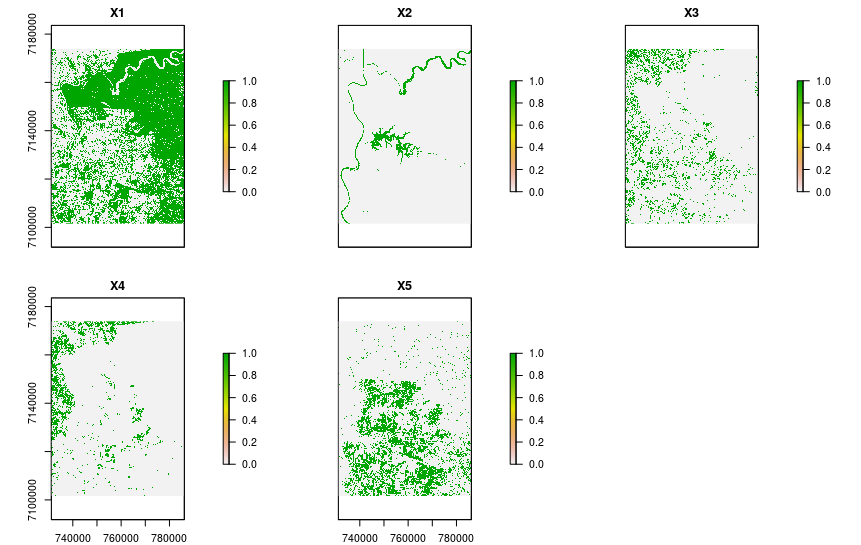
\includegraphics{clases_5.png}
      \caption{Clases generadas por el algoritmo kmeans para 5 clases.}
      \label{fig:clases5}
    \end{figure}
    Abriremos la imagen ahora en el qgis e identificaremos cada una de las clases realiando interpretacion visual de la imagen.

    Para realizar la identificacion primero vamos al menu \menu{propiedades de la
    imagen, Estilo, Tipo de renderizacion, Unibanda pseudocolor}. Elegimos de modo
    Intervalo Igual y en numero de clases ponemos con el minimo en 1 y el maximo en
    5. En estilo de color elegimos colores aleatorios. Iremos luego cambiando los
    colores uno a uno por un color brillante e identificado a que cobertura
    pertenece dicha clase espectral.

    Construiremos con ella una tabla como la siguiente

    \begin{verbatim}
        id  class
        1   2
        2   7
        3   1
        4   1
        5   1
    \end{verbatim}

  que guardaremos en un archivo de texto con el nombre \file{class}. El mismo lo utilizaremos para realizar
  la fusion de clases.

  Una vez conocidas las categorias de uso y cobertura correspondientes a cada
  clase espectral podemos combinarlas

  \begin{lstlisting}
      clases.2016 <- read.delim("aux_data/class.txt")
      reclas.2016 <- subs(kmeans.2016$map, clases.2016)
  \end{lstlisting}

  para graficar ahora con los colores prestablecidos definimos la paleta de colores y fijamos los limites

  \begin{lstlisting}
    colores = c('#b2df8a','#33a02c',
                '#fdbf6f','#ff7f00',
                '#fb9a99','#e31a1c',
                '#a6cee3','#1f78b4')
    plot(reclas.2016, col=colores, zlim=c(1,8))
  \end{lstlisting}
  \begin{figure}
    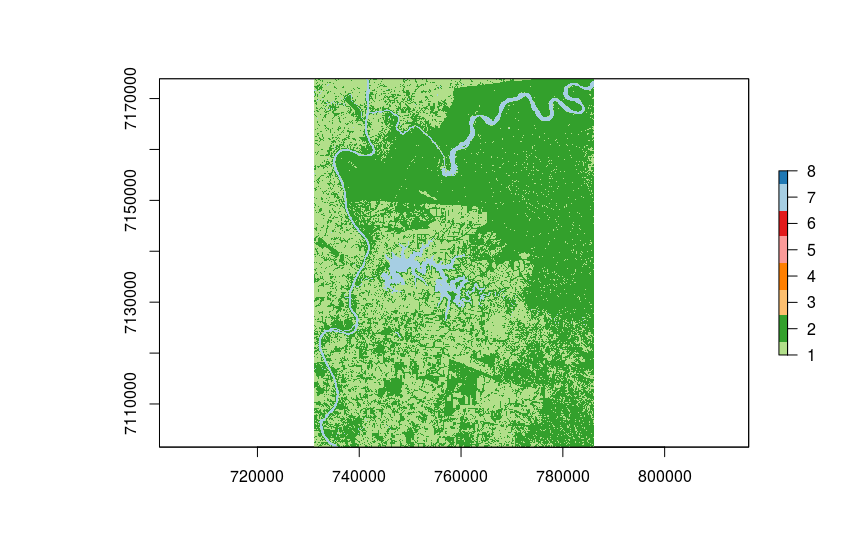
\includegraphics{kmeans-colores.png}
    \caption{Imagen clasificada por el metodo kmeans con 5 clases.}
    \label{fig:kmean5}
  \end{figure}
\end{exa}

\begin{exa}
  Hagamos un analisis espectral de las imagenes clasificadas antes y despues de la fusion.
  Para esto utilizaremos a la imagen clasificada como mascara para asignar los colores
  al scatterplot. Para esto usaremos la libreria \texttt{rasterVis}.

  Agregamos la imagen clasificada a las bandas de la imagen en reflectancia y luego
  hacemos los scatterplot segun la clase espectral o de informacion como

  \begin{lstlisting}
    stack.2016 <- stack(ref.2016, reclas.2016)
    xyplot(nir+swir1~red, groups=MC_ID, data=stack.2016)
  \end{lstlisting}
  Vemos que las clases espectrales pueden unirse en clases de informacion y que algunas clases de informacion no se separan en distintas clases espectrales (figuras \ref{fig:esk}).
  \begin{figure}
    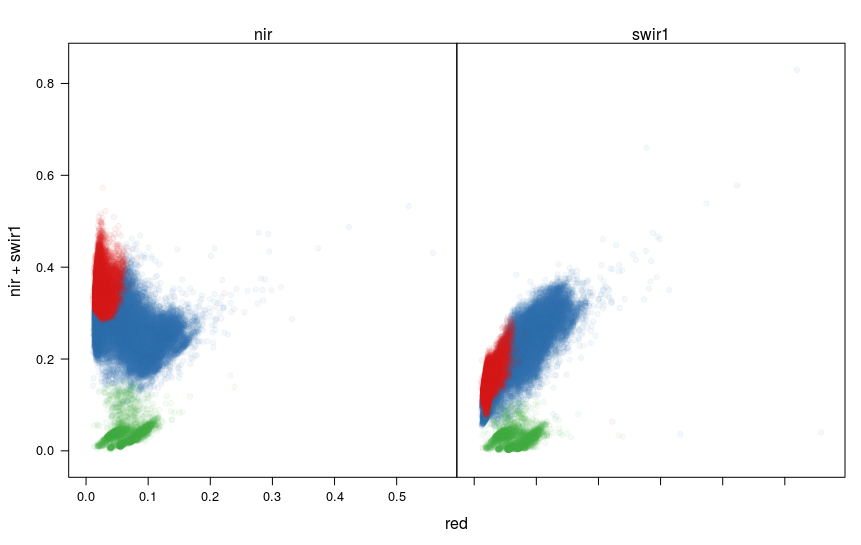
\includegraphics{kmeans-es.png}
    \caption{Espacio espectral clasificado por kmeans.}
    \label{fig:esk}
  \end{figure}

\end{exa}

\begin{exa}
  Repitamos este analisis pero con 100 clases espectrales. El algoritmo es el mismo
  pero ahora vamos a usar el parametro nClasses igual a 100.
  \begin{lstlisting}
  set.seed(42)
  kmeans.2016b <- unsuperClass(ref.2016, nClasses = 100, nStarts = 100,
                              nSamples = 1000)
  writeRaster(kmeans.2016b$map, "raster_data/processed/kmeans2016b",
              datatype="INT1U", overwrite=TRUE)
  clasesb.2016 <- read.delim("aux_data/class100.txt")
  reclasb.2016 <- subs(kmeans.2016b$map, clasesb.2016)
  plot(reclasb.2016, col=colores, zlim=c(1,8))
  \end{lstlisting}

  \begin{figure}
    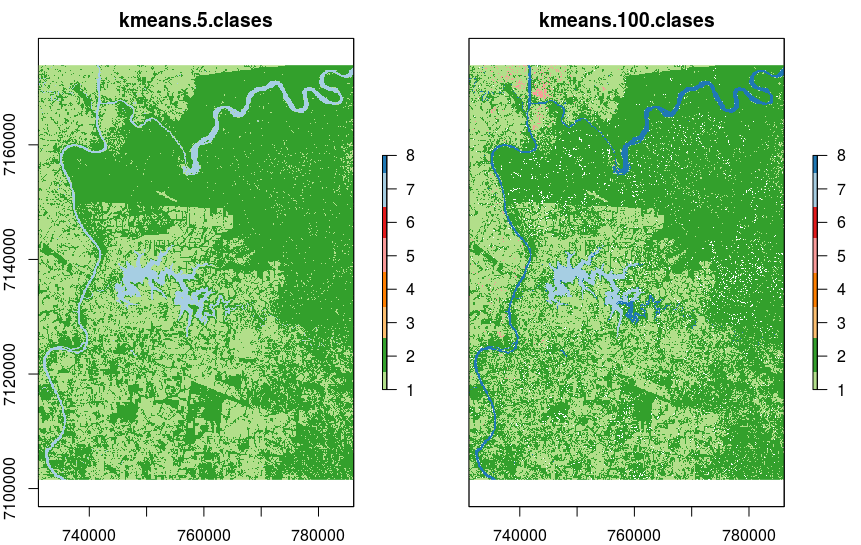
\includegraphics{5v100.png}
    \caption{Comparacion entre la clasificacion con 5 clases y 100 clases espectrales.}
    \label{fig:5v100}
  \end{figure}

  Comparamos nuevamente los espacios de fase entre la clasificacion obtenida a partir de 5 y 100 clases espectrales
  \begin{lstlisting}
    stackb.2016 <- stack(ref.2016, reclasb.2016)
    xyplot(nir+swir1~red, groups=MC_ID, data=stack.2016)
    xyplot(nir+swir1~red, groups=MC_ID, data=stackb.2016)
  \end{lstlisting}

  Vemos en este caso que somos capaces de separar todas las clases de informacion en el espacio de fases.

\end{exa}

\begin{act}
    Vuelva a repetir la clasificacion utilizando la imagen obtenida de la transformada por componentes principales descartando las bandas que aporten menos informacion.
\end{act}

\begin{act}
  Repita la clasificacion para la imagen landsat 7 del año 2000.
\end{act}


\section{Informacion espacio-temporal}
Con el fin de mejorar la clasificacion podemos incorporar informacion espacial y temporal a la informacion radiometrica. De esta forma estaremos, al momento de clasificar los pixeles, ya no trabajando en un espacio espectral si no en uno mas amplio. Veamos como hacer esto.

\begin{exa}
  Para incorporar informacion espacial sobre el contexto del p\'ixel, podemos
  hacerlo tanto antes como despu\'es de la clasificaci\'on. Nos centraremos
  en este caso en como hacerlo antes.

  Calculamos primero la variabilidad local de brillo para la banda pancromatica
  de la imagen Landsat 8 como

  \begin{lstlisting}
    pan.2016 <- raster("raster_data/LC82240782016304LGN00/LC82240782016304LGN00_B8.TIF")
    window <- matrix(1,nrow=5, ncol=5)
    sd.2016<-focal(pan.2016,w=window,fun=sd)
    plot(log(sd.2016,base = 10), zlim=c(1,4))
  \end{lstlisting}

  Vemos que las zonas con mayor presencia de urbanizaciones presentan una mayor variabilidad que aquellas con menor presencia.

  \begin{figure}
    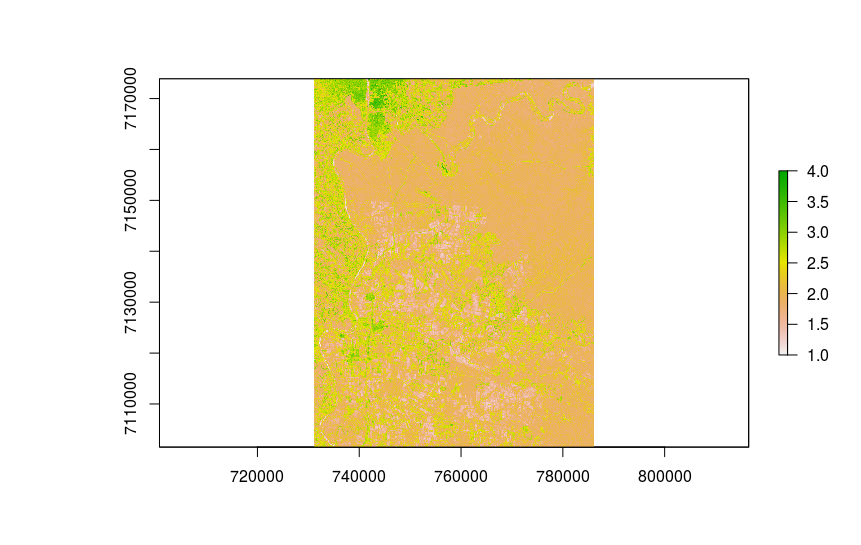
\includegraphics{pan-sd.png}
    \caption{Desvio standar para una ventana de 5 pixeles por 5 pixeles en escala logaritmica.}
    \label{fig:pansd}
  \end{figure}

  Una vez obtenida la banda de desvio standar, podemos agregarla a las demas, luego
  de remuestrearla haciendo

  \begin{lstlisting}
    sd.2016 <- aggregate(sd.2016, fact=2, fun=mean)
    stack(ref.2016, sd.2016)
    pca.2016 <- rasterPCA(stack(ref.2016, sd.2016), spca = TRUE)
  \end{lstlisting}

  \begin{Verbatim}[fontsize=\small]
  Importance of components:
                            Comp.1    Comp.2    Comp.3     Comp.4      Comp.5      Comp.6      Comp.7
  Standard deviation     2.1592402 1.1821570 0.8392878 0.40888073 0.196591748 0.143753334 0.096362617
  Proportion of Variance 0.6660455 0.1996422 0.1006292 0.02388335 0.005521188 0.002952146 0.001326536
  Cumulative Proportion  0.6660455 0.8656876 0.9663168 0.99020013 0.995721318 0.998673464 1.000000000
  \end{Verbatim}

  Vemos en este caso, analizando el sumario, que la banda de textura agrega informacion
  con respecto a la solo disponible al utilizar las bandas en radiancia.
\end{exa}

\begin{act}
  Repita el ejemplo para la imagen landsat 7 del año 2000. Clasifique por el metodo de kmeans las imagenes de los años 2000 y 2016.
\end{act}

\begin{exa}
  Para incorporar informacion del contexto temporal, agregaremos a la informacion
  espectral informacion sobre la variacion del indice de vegetacion durante el
  año en que se tomo la imagen. Primero cargamos las imagenes modis del 2016

  \begin{lstlisting}
    list.2016 <- list.files("raster_data/MOD13Q1/NDVI/", pattern = "MOD13Q1.A2016+.*tif", full.names = TRUE)
    ndvi.2016 <- stack(list.2016)/1e4
    ndvi.2016 <- approxNA(ndvi.2016)
    sd.2016 <- calc(ndvi.2016, fun = sd)
    me.2016 <- calc(ndvi.2016, fun = mean)
    plot(stack(me.2016,sd.2016))
  \end{lstlisting}

  Una vez hecho esto, resampleamos el promedio y el desvio de la serie temporal
  y lo unimos a las imagenes en reflectancia, sobre las cuales calcularemos
  la transformada por componentes principales.

  \begin{lstlisting}
    sd.2016 <- resample(sd.2016, ref.2016, method="ngb")
    me.2016 <- resample(me.2016, ref.2016, method="ngb")
    pca.2016 <- rasterPCA(stack(ref.2016, me.2016, sd.2016), spca = TRUE)
    summary(pca.2016$model)
  \end{lstlisting}

  podemos ahora seleccionar las 4 componentes que explican el 99\% de comportamiento de la imagen y clasificarla.

  \begin{Verbatim}[fontsize=\small]
    Importance of components:
                              Comp.1    Comp.2     Comp.3     Comp.4     Comp.5      Comp.6      Comp.7      Comp.8
    Standard deviation     2.3109360 1.3111953 0.69083373 0.48042475 0.41555630 0.176127381 0.139538990 0.095410787
    Proportion of Variance 0.6675532 0.2149042 0.05965641 0.02885099 0.02158588 0.003877607 0.002433891 0.001137902
    Cumulative Proportion  0.6675532 0.8824573 0.94211373 0.97096472 0.99255060 0.996428206 0.998862098 1.000000000
  \end{Verbatim}
\end{exa}

\begin{act}
  Repita el ejemplo para la imagen Landsat 7 del año 2000. Clasifique por el metodo de kmeans las imagenes de los años 2000 y 2016.
\end{act}
